\chapter[Epigenetics: Same Sequence, Different Uses]{Epigenetics:\protect\\ Same Sequence, Different Uses}

\begin{kaichang}
Do not spread that honey from the kitchen on your bread just yet. Think about where it came from: a hive houses one queen and tens of thousands of workers. The queen has fully developed ovaries, can lay over a thousand eggs a day, and may live for several years; workers are also female, yet have almost no reproductive capacity, live only a few dozen days in summer, and spend their lives gathering nectar, building the hive, and caring for larvae.

Here is the key: a queen and workers can be daughters of the same queen, with almost identical genomes. What sends them toward completely different destinies is not their gene sequences---it is what they eat as larvae. A larva fed royal jelly throughout develops into a queen; one fed royal jelly for only two or three days before switching to honey and pollen becomes a worker.

How can the same blueprints produce two different buildings? Stranger still, once built, each building can ``remember'' its form, yet be demolished and rebuilt when necessary. In this chapter, we will unpack the annotation system written on top of DNA without altering DNA itself.
\end{kaichang}

\section{The Same Blueprints, Different Lives}

Before jumping to conclusions, let us examine a few more phenomena that can be observed and measured.

You already know the bee example. Now consider identical twins: they develop from a single fertilized egg, have almost exactly the same sequences, and look so alike as children that people cannot tell them apart. Decades later, however, one has smoked for years while the other exercises outdoors regularly, and their blood pressure, skin, and chronic disease risks may differ enormously. Test their DNA, and the sequences are still the same sequences.

Then consider cats. Calico and tortoiseshell cats have irregular patches of black, orange, and white, and almost all are female. More intriguing still is the cloned cat ``CC,'' born in 2001: all its DNA was copied from a tricolored female, yet its coat pattern differed markedly from the ``original.'' The sequence was identical, but the pattern was not photocopied.

There is also you. When a cut heals, the new cells are skin cells, never liver cells or neurons. Stem cells in your body divide for decades, and their descendants always ``remember'' who they are. Meanwhile, a caterpillar inside its pupa is almost completely dismantled and reassembled into a butterfly---without a single letter of its genome changing from start to finish.

Pea aphids provide another example: females can produce daughters without mating. Daughters from the same batch remain wingless when food and space are plentiful; when crowding and hunger set in, the offspring grow wings to prepare for a move. The genome is still the same, with different developmental switches flipped in response to the environment.

All these phenomena share one feature: \textbf{the DNA sequence stays the same, but the way genes are used changes, and that change can persist}. Chapter 70 explained that transcription factors and chromatin accessibility determine whether a gene is on at a given moment. But it left one question unanswered: how can cells remember an ``open or closed'' state and pass it down through successive generations of descendants? The answer lies with this chapter's central character.

\section{Zooming In on Chromosomes}

Recall the picture from Chapter 66: your DNA is two meters long when stretched out, yet must fit into a nucleus less than one-hundredth of a millimeter across. It does so through successive layers of packaging---DNA winds like thread around histone ``spools'' to form nucleosomes, which fold and coil into chromatin. Where the winding is tight, the transcription machinery cannot squeeze in, and genes remain silent; where it is loose, promoters (Chapter 68) are exposed, giving genes a chance to be read.

Epigenetic annotations primarily consist of two kinds of chemical marks applied to this packaging system.

\textbf{The first kind: DNA methylation.} An enzyme attaches a methyl group (\chem{CH_3}) to carbon 5 of cytosine (C), producing 5-methylcytosine. This happens almost exclusively where ``C is followed by G,'' written CpG. Where does the methyl group come from? A molecule called SAM delivers it---the cell makes this general-purpose ``methyl donor'' from methionine. Notice that none of the four letters A, T, G, and C has changed; some Cs simply acquire a little chemical ``hat.''

\textbf{The second kind: histone modification.} Histones have flexible ``tails'' that protrude from nucleosomes. Small groups such as acetyl and methyl groups can be attached to amino acids, including lysine, on these tails. Acetylation neutralizes lysine's positive charge, weakening its electrostatic attraction to negatively charged DNA and loosening the winding. Histone methylation is subtler: on the same tail, different positions and different proteins that read the mark can produce either an on or an off effect.

There is also a third operation: chromatin-remodeling complexes use ATP energy to shift entire nucleosomes or exchange histone variants. Together, these three approaches form chromatin's ``annotation language.''

\begin{table}[htbp]
\centering
\begin{tabular}{lll}
\toprule
Mechanism & Site & Typical effect \\
\midrule
DNA methylation & Cytosine in CpG & \shortstack[l]{High promoter methylation\\usually suppresses transcription} \\
\shortstack[l]{Histone\\acetylation} & \shortstack[l]{Lysine on\\histone tails} & \shortstack[l]{Loosens chromatin; tends\\to promote transcription} \\
\shortstack[l]{Histone\\methylation} & \shortstack[l]{Specific positions\\on histone tails} & \shortstack[l]{On or off, depending on\\position and reader proteins} \\
\shortstack[l]{Chromatin\\remodeling} & Whole nucleosomes & \shortstack[l]{Moves or replaces nucleosomes,\\changing accessibility} \\
\bottomrule
\end{tabular}
\end{table}

One point deserves emphasis: these mechanisms adjust probabilities; they are not infallible switches. Heavy methylation of a promoter makes it \textbf{harder} to transcribe, rather than physically locking a door. Whether a gene ultimately turns on, and how strongly, also depends on the transcription-factor network discussed in Chapter 70. Expression level is a continuous variable; annotations alter its range of possible values.

Another important detail: roughly six in ten human genes have a CpG-rich region near their promoter, called a CpG island. In healthy cells, these islands usually remain lightly methylated, leaving genes ``available.'' Abnormal methylation of an island may silence its corresponding gene for a long time---you will encounter this pattern again when we discuss cancer. By contrast, methylation within a gene's coding region often coexists with active expression. Clearly, ``methylation means off'' is only a rough mnemonic: where an annotation lands is part of its meaning.

This annotation system is also ``alive,'' maintained by a complete set of enzymes: ``writers'' add methyl groups, ``erasers'' gradually oxidize and ultimately remove them, and ``readers'' recognize particular marks and recruit other proteins. These three classes of proteins make annotation a dynamic process: a cell can remember a state for a long time yet rewrite it precisely when a signal arrives. For example, hormones or developmental signals can dispatch ``erasers'' to specific genes, remove silencing annotations, and return those genes to the available list. The regulatory network in Chapter 70 makes the ``decisions''; this chapter's annotation system ``files them away.''

\begin{shiyan}
\textbf{Observing ``One Genome, Two Colors''}

Materials: one garlic bulb, two shallow dishes, clean water, and an opaque cardboard box.

Procedure: peel the garlic cloves, divide them between the dishes, and add a little water without submerging them. Put one dish on a windowsill in the light and cover the other with the box to exclude light. Top up the water daily and observe for one to two weeks.

What to observe: the illuminated group grows green shoots; the shaded group grows tender yellow ``blanched garlic shoots''---both are actually sold in vegetable markets. The shoots in the two dishes have exactly the same DNA sequences; their colors differ because light activates or suppresses the expression of genes involved in chlorophyll synthesis. Bring the yellow shoots into the light, and they turn green after a few days: the switch is reversible.

Strictly speaking, this light switch mainly relies on the transcriptional regulation discussed in Chapter 70. Plants do, however, use epigenetic annotations to ``remember'' their environment: winter wheat must experience winter cold before heading and flowering (vernalization). Cells use histone marks to keep a flowering-inhibitor gene switched off for a long time, creating a memory of the cold.

Safety reminder: this experiment involves no hazardous operations. Just remember that moldy or spoiled garlic must not be eaten, and discard the experimental materials afterward.
\end{shiyan}

\section{Passing Annotations to Daughter Cells}

Now we can answer the chapter's central question: how is memory maintained?

Replication creates the difficulty. Before a cell divides, DNA replicates semiconservatively (Chapter 67): an old strand remains, while the new strand is freshly synthesized---and none of the cytosines on that new strand has a methyl group. Left unattended, methylation annotations would be diluted by half with every division and disappear after a few generations.

The cell's solution is a ``copyist'': maintenance DNA methyltransferase (DNMT1). It specifically recognizes hemimethylated CpGs, where ``the old strand has a methyl group but the new one does not,'' and adds methyl groups at corresponding positions on the new strand, following the old strand's pattern. The methylation pattern is thus recopied at every cell division: descendants of dividing skin stem cells remain skin cells, decade after decade.

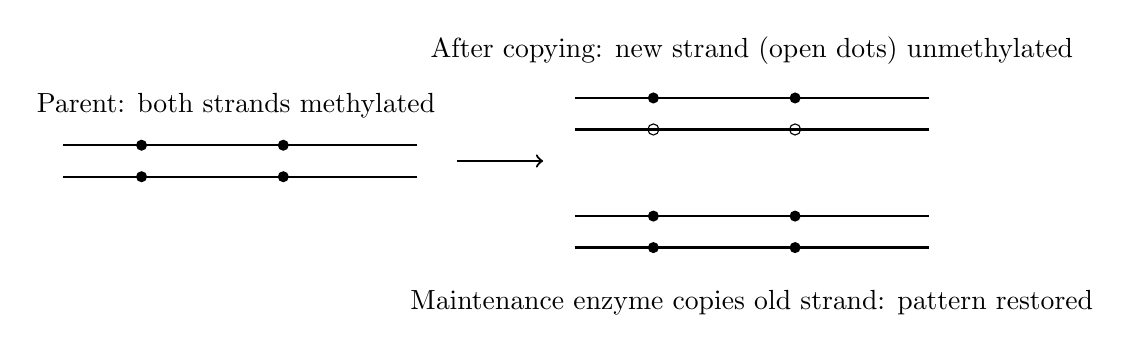
\begin{tikzpicture}
\draw[thick] (0,1.6)--(4.5,1.6);
\draw[thick] (0,1.2)--(4.5,1.2);
\fill (1,1.6) circle (2pt); \fill (2.8,1.6) circle (2pt);
\fill (1,1.2) circle (2pt); \fill (2.8,1.2) circle (2pt);
\node at (2.2,2.1) {Parent: both strands methylated};
\draw[->,thick] (5.0,1.4)--(6.1,1.4);
\draw[thick] (6.5,2.2)--(11,2.2);
\draw[thick] (6.5,1.8)--(11,1.8);
\fill (7.5,2.2) circle (2pt); \fill (9.3,2.2) circle (2pt);
\draw (7.5,1.8) circle (2pt); \draw (9.3,1.8) circle (2pt);
\node at (8.75,2.8) {After copying: new strand (open dots) unmethylated};
\draw[thick] (6.5,0.7)--(11,0.7);
\draw[thick] (6.5,0.3)--(11,0.3);
\fill (7.5,0.7) circle (2pt); \fill (9.3,0.7) circle (2pt);
\fill (7.5,0.3) circle (2pt); \fill (9.3,0.3) circle (2pt);
\node at (8.75,-0.4) {Maintenance enzyme copies old strand: pattern restored};
\end{tikzpicture}

(Filled dots represent methyl marks, and lines represent DNA strands. This is a schematic convention: real DNA is a double helix, and methyl groups are too small to see with the naked eye.)

How accurate is this copying system? That question is the key to understanding epigenetics as a whole.

\begin{qiaoliang}
Let us do the arithmetic. The human genome has about 28 million CpG sites, most of which are methylated in most cells. Experiments estimate maintenance-copying fidelity at roughly 96\%--99\% per site per division. That sounds high, but take 99\% and calculate: the probability that a site remains unchanged after 50 cell divisions is about $0.99^{50}\approx 0.61$. In other words, by adulthood, annotations at a substantial fraction of sites in your body have already ``drifted.'' (Cells also contain enzymes that actively demethylate DNA and erase annotations, so the drift is not entirely random.)

Compare this with Chapter 72's number: the DNA sequence mutation rate is on the order of $10^{-8}$ per base per generation. Epigenetic annotations have an error rate thousands or tens of thousands of times higher than sequence mutation. That captures the system's essential character: it is an \textbf{erasable, flexible, but not very reliable} whiteboard, suited to recording ``this cell's current operating manual,'' not to storing an archive for posterity. Information that must last billions of years still has to be engraved in DNA sequence.
\end{qiaoliang}

X-chromosome inactivation provides another striking example. Female mammals have two X chromosomes, giving them twice the male gene dosage. Each early embryonic cell randomly ``archives'' one X, compressing it into an almost nonexpressing ``Barr body'' and maintaining that state for life through methylation and other annotations, which are passed on during division. Crucially, each cell's choice of which X to archive is random. Calico coat-color genes happen to lie on the X chromosome: cells that archive the ``black X'' produce orange fur, and those that make the opposite choice produce black fur, assembling a random patchwork across the cat. This also explains why the clone CC had a different pattern: the donor nucleus used for cloning had already chosen ``which X to archive,'' so the pattern naturally failed to match the original. Calicos are almost all female because this patchwork requires two X chromosomes.

\section{Evidence from a Multicolored Mouse Litter}

The claim that annotations can change traits requires experiments, not logic alone. The following story is classic evidence in epigenetics; its design, checks, and controversies deserve a close look.

\begin{zhengju}
\textbf{Question.} A type of ``agouti'' mouse carries a special allele, $A^{vy}$. Strangely, genetically identical littermates range in coat color from pure yellow to brown, and even differ in body weight: yellow individuals tend to be obese and susceptible to diabetes. Why do identical genotypes produce different traits?

\textbf{Clue.} Sequencing revealed a virus-derived ``jumping sequence'' (a transposon) inserted upstream of $A^{vy}$. Like an uncontrolled switch, it makes the coat-color gene express itself at the wrong times and places. Methylation measurements then showed high methylation and low expression at this site in brown mice, but low methylation and high expression in yellow mice. Identical sequences, different annotations.

\textbf{Experiment.} In 2003, Waterland and Jirtle added methyl donors---folic acid, vitamin B12, choline, and betaine---to pregnant mice's feed. The proportion of brown offspring increased significantly. In other words, diet during pregnancy altered offspring coat color and metabolism by influencing methylation in early embryos.

\textbf{Checking alternative explanations.} Could the methyl donors directly induce sequence mutations? Sequencing ruled that out. Could toxicity explain the effect? The doses were far below the toxic range, and the effect was concentrated at specific loci. Could this merely be a general effect of the uterine environment? Later embryo-manipulation experiments narrowed the window of action to the early embryo---precisely when genome-wide annotations undergo large-scale rewriting.

\textbf{Debate and refinement.} Many such ``diet changes epigenetics'' experiments have small samples and depend on special sequences such as transposons; similar arrangements are rare in the human genome. Their conclusions therefore cannot be extrapolated to ``what a pregnant woman eats determines her child's gene switches for life.'' The experiment's defensible conclusion is that environmental influences can alter epigenetic annotations early in development, and differences in those annotations can stably change traits. That alone is remarkable enough.
\end{zhengju}

\textbf{Translator safety note:} This mouse experiment is not a supplement regimen for people. Do not change pregnancy supplements to manipulate a child's traits; discuss supplements with a qualified prenatal clinician. This caution does not negate established folic-acid recommendations for preventing neural-tube defects. See \href{https://ods.od.nih.gov/factsheets/Pregnancy-HealthProfessional/}{NIH pregnancy nutrition guidance}.

\section{Where the System's Limits Lie}

Every model has a range of applicability. Epigenetics especially needs clear boundaries, because few fields are exaggerated more often.

\textbf{Limit one: two ``great cleanups.''} During the mammalian life cycle, genome-wide methylation undergoes two major resets: one in the early embryo after fertilization, and another during germ-cell formation, when old imprints are erased and rebuilt according to the individual's sex. The vast majority of acquired annotations cannot survive these two checkpoints. That is actually beneficial: each generation can start with a nearly clean slate instead of carrying all its ancestors' ``wear marks.''

\textbf{Limit two: exceptions exist, but they are special cases.} Genomic imprinting is one officially permitted exception: humans have roughly a hundred or more genes bearing ``paternal'' or ``maternal'' labels that escape part of the resetting. For example, \emph{IGF2} is usually expressed only from the father's copy. This demonstrates that carrying annotations across generations is mechanistically possible, but involves a strictly regulated minority. Plants have broader limits: their resetting is less thorough than mammals', making epigenetic variation easier to transmit for several generations. A particularly elegant example is toadflax: an altered flower shape, from bilateral to radial symmetry, was recorded as far back as Linnaeus's time. In 1999, scientists showed that it reflected methylation-induced silencing of \emph{Lcyc}, not a sequence mutation. It can persist for several generations, occasionally reverting spontaneously. This is a genuine natural ``epimutation,'' yet it also exposes epigenetics' weakness: it is less stable than sequence and can switch back on its own.

\textbf{Limit three: human transgenerational evidence needs careful interpretation.} The most famous case is the Dutch ``Hunger Winter.'' Children born to mothers who went hungry during pregnancy in the famine of 1944--1945 showed small methylation differences in certain genes, such as \emph{IGF2}, decades later, along with slightly higher cardiometabolic risks. But note two things: the effects are small; and during pregnancy, both the fetus and its developing germ cells were directly affected by famine. Strictly speaking, this is not transgenerational inheritance, but ``direct exposure of two generations at once.'' To establish transmission to unexposed grandchildren or great-grandchildren, existing human studies offer weak effects and too many confounders: family environments and dietary traditions also pass down generations and are difficult to disentangle. The honest conclusion is that genuine transgenerational epigenetic inheritance in humans \textbf{may exist, but remains unresolved}. Evidence is firmer in plants and lower animals, but cannot simply be transferred to humans.

\textbf{Limit four: it has overthrown no one.} DNA sequence remains the only molecule proven to carry information stably across tens of millions of years. Mendel's laws still describe allele segregation: however elaborate the annotations in $A^{vy}$ mice, the allele itself is still inherited in Mendelian fashion. Natural selection acts on heritable phenotypic differences; if an epigenetic variant is heritable, it too can be selected. Its low fidelity simply makes it unlikely to replace sequence variation in evolution's long-distance race. Epigenetics adds a layer of ``rewritable memory'' to gene regulation: it is a \textbf{supplement}, not a revolution.

\begin{wuqu}
``Epigenetics proves Lamarck right: the muscles you build, the trauma you suffer, even your thoughts can be written into genes and passed to your descendants.'' This is the most widespread overextension of epigenetics.

Counterexamples and facts: first, mammalian germ cells undergo extensive resetting, so most acquired annotations never reach the next generation; your muscle memory stays in your own muscles. Second, studies claiming human ``transgenerational epigenetics'' generally find tiny effects and can almost never exclude more ordinary explanations: children in traumatized families live in environments shaped by trauma, and environment and culture themselves pass between generations without invoking DNA. Third, even in plants and lower animals, where evidence is stronger, transgenerational epigenetics is probabilistic, reversible, and limited to a few generations, not ``unrestricted rewriting followed by stable inheritance.'' Your experiences may indeed fine-tune annotations in some cells and affect your own body, but there is currently no evidence for ``inheritable thoughts.'' Science is at its most honest when it openly admits what remains unknown.
\end{wuqu}

\section{Back to the Honey Jar}

We can now answer the opening question in full. In 2008, researchers used RNA interference, a technique related to the regulatory RNAs mentioned in Chapter 68, to reduce DNA methyltransferase in honeybee larvae. Most larvae that should have become workers developed well-formed ovaries and shifted toward queen development. The methylation system is one of the mechanisms executing that fork in developmental fate. Components of royal jelly influence early larval epigenetic annotations, as well as hormonal signals, steering the same genome toward a different operating plan.

Notice another detail: daughters of workers can still become queens if fed royal jelly again. Annotations can be rewritten; the blueprints never changed. That is what ``epigenetic'' means: a layer of regulation above the genes, with epi- meaning ``above.''

The twins' mystery is also resolved: their annotations are highly similar at birth, but age, diet, smoking, and other differences cause those annotations to drift apart. Sequencing still finds the same sequence, yet the methylation maps differ.

\section{Rewritable Marks as Drug Targets}

The rewritability of epigenetic annotations is a medical opportunity.

Cancer cells show a characteristic annotation disorder: widespread loss of genome-wide methylation, which destabilizes chromosomes, alongside local hypermethylation that forcibly silences tumor-suppressor genes. If annotations rather than missing sequence cause the silencing, reversal may be possible. Once incorporated into DNA, azacitidine and decitabine ``trap'' methyltransferases, forcing cells to reduce methylation and returning silenced tumor-suppressor genes to work. They are already standard treatments for myelodysplastic syndromes and certain leukemias. Another drug class inhibits histone deacetylases, altering annotations from the histone side.

\textbf{Translator safety note:} These are specialist cancer treatments, not self-directed ways to reset genes or slow aging. Azacitidine is a hazardous drug that can suppress blood-cell production and harm a fetus; its use requires clinical monitoring and appropriate handling. See the \href{https://dailymed.nlm.nih.gov/dailymed/fda/fdaDrugXsl.cfm?setid=80a43736-0598-4e4b-85ba-e29daa290c8f\&type=display}{official azacitidine prescribing information}.

Another popular application is the ``epigenetic clock.'' In 2013, Horvath discovered that methylation levels at several hundred CpG sites could predict a person's biological age fairly accurately; these clocks are now widely used in aging research. Interpretation requires caution, though: a clock is a statistical correlation, and turning its hands backward does not necessarily reverse aging itself.

Problems with imprinted genes can also directly cause disease. A region on chromosome 15 silences different genes on its paternal and maternal copies. Loss of the paternal region causes Prader--Willi syndrome, with weak muscles and an appetite that is never satisfied; loss of the maternal region causes the quite different Angelman syndrome, with developmental delay and frequent laughter. The same chromosome region produces completely different consequences depending solely on whether it came from the father or mother---solid evidence of genomic imprinting in humans.

One major reason animal cloning has a low success rate is that the egg cannot completely reset the donor nucleus's annotations in time. Conversely, induced pluripotent stem-cell technology, which ``washes'' ordinary body cells back into stem cells, essentially erases their epigenetic memory artificially.

That raises one last question: after annotations are reset to a nearly blank slate, how does a fertilized egg start from scratch and use gene-regulatory networks to draw an entire body's blueprint step by step---first distinguishing head from tail, then specifying limbs, and finally putting three trillion cells in their proper places? That is the next chapter's story: Chapter 75, ``From a Fertilized Egg to a Body.''

\begin{tiaozhan}
Histone tails have dozens of modifiable sites and more than ten kinds of modifications, creating an astronomical number of theoretical combinations. This inspired the ``histone code'' hypothesis: these combinations form a code that specific proteins read, one by one, to determine genes' fates. The hypothesis remains controversial. Critics note that many histone marks are consequences, not causes, of transcription: genes turn on first and marks follow. Furthermore, the same mark at the same site is read differently in different cell types, and correlation is not causation. A more cautious current picture treats epigenetic marks as components and memory carriers of regulatory networks, participating in feedback loops rather than constituting an independent code that can be translated word for word. Science has no final answer here---that is exactly what a research frontier looks like. You can skip this section without losing the main thread.
\end{tiaozhan}

\section*{Try It Yourself}

\begin{sikaoti}
\item Draw an information-flow diagram from ``larva eats royal jelly'' to ``develops into a queen,'' connecting environmental signal, epigenetic annotations, gene expression, and developmental outcome with arrows. Indicate where the DNA sequence appears in the process. (Hint: it remains unchanged throughout.)
\item Use semiconservative replication to explain why methylation marks can persist across cell divisions whereas ``a protein's own folded shape'' usually cannot. Draw the old and new strands after replication and show where maintenance DNA methyltransferase acts.
\item Estimate: if a CpG site has a 0.98 probability of remaining unchanged at each cell division, what is the approximate probability that it remains unchanged after 100 divisions? (Hint: $0.98^{100}$; use $\ln 0.98\approx -0.02$ to estimate.) Compare this with a sequence mutation rate of about $10^{-8}$ per base per generation. What tasks suit epigenetic annotations, and what tasks do not?
\item Almost all calico cats are female. Explain why using X-chromosome inactivation, and predict whether a cat cloned from a calico's body cell would have exactly the same coat pattern. Why or why not?
\item After reading a report that ``a mother's diet changes mouse coat color,'' a classmate says, ``So what my mother ate during pregnancy determined my genes for life.'' Identify at least two imprecise aspects of this claim.
\item Design a distinguishing experiment: you discover a heritable variant in a plant trait and want to know whether it reflects a sequence mutation or an epimutation. List two tests that could distinguish them and explain the principle behind each. (Hint: sequencing; checking whether the trait reverts after treatment with a demethylating drug.)
\end{sikaoti}

\textbf{Translator safety note:} Keep the drug-treatment exercise a paper design. Do not obtain or apply demethylating cancer drugs to home or classroom plants; any real study belongs in an appropriately equipped, supervised laboratory after formal risk assessment. See the \href{https://dailymed.nlm.nih.gov/dailymed/fda/fdaDrugXsl.cfm?setid=80a43736-0598-4e4b-85ba-e29daa290c8f\&type=display}{azacitidine hazards} and \href{https://institute.acs.org/acs-center/lab-safety/education-training/safer-experiments.html}{ACS experiment-safety guidance}.
